
\typeout{new file: Using_RADCAL_Chapter.tex}

\chapter{Using RadCal}
\label{chap::using_RADCAL}

This chapter describes in details how to compile RadCal, how to write an input file using the namelist formatting, how to run RadCal, and describes the output files. Important modifications were brought to the code since it last release in 1993 \cite{Grosshandler1993}. In particular, the input file has been completely upgraded and the user who wishes to use this new version of the code must rewrite the old RadCal input file to comply with the new syntax.

\section{Compiling RadCal}

This new version of RadCal is a Fortran 2008 written software, written following modular paradigm. A complete description of the code is presented in Chapter~\ref{chap:Code}. The source code is contained in the file \verb=RADCAL.f90=. It includes the RADCAL module and the main program.

The file \verb=Makefile= is the make file to compile \verb=RADCAL.f90= and to generate the executable \verb=RADCAL.x=. It is made for Linux machine using the Intel Fortran compiler (\verb=ifort=). It has a couple of flags. Typing \verb'make DEBUG=0' will compile RADCAL using the compiler optimization flags. Typing \verb'make DEBUG=1' will compile the code in debugging mode. This is useful to detect any error or bug when the source file is modified. In debug mode, the code displays additional data on the screen. It prints the pressure (in atm), physical length (in cm), the temperature (in K) of each segment that composes the domain. It also prints on screen the values contained of the Lorentz half-width at half-maximum $\gamma_c$ vector for each species included in RadCal. Furthermore, it also prints characteristics pertaining to $\rm CO_2$ if this species is included in the calculation and if the wavenumber $3600~\rm cm^{-1}$ is included in the user defined spectrum. It is recommended to use RadCal with the optimizing flag as it is slightly faster than the debugging mode.

In addition to the optimization flag, a second flag enabling the compilation of the code with \verb=OpenMP= (for loop parallelization) has been implemented. To compile the code with \verb=OpenMP=, just type \verb'make DEBUG=0 PARALL=1' (for optimization version) or \verb'make DEBUG=1 PARALL=1' for the debugging \verb=OpenMP= version. Note that the \verb=OpenMP= version does not improve much the performances, but it was included there for experimentation.

\section{Input file}

The input file is named \verb=RADCAL.in=. The input file format has changed since the last RADCAL version. It now uses the Fortran \verb=namelist= formalism, which is more convenient. What is needed is the knowledge, for each segment along the line of sight, of the local temperature (\verb=T=), distance (\verb=LENGTH=), pressure (\verb=PRESSURE=), soot volume fraction (\verb=Fv=), and species mole fraction, (\verb=X<species name>=).
\textbf{It is very important that the sum of all the species mole fraction over a given segment is equal to 1}. Otherwise the code will not compute and will return an error message in the output file \verb=RADCAL.out=.

A list of all the RadCal available species is included in the code and is printed in a automatically generated \verb=RADCAL.in= in the case the user did not provide any input file. Unlike the old version, you can now solve the radiative Transfer Equation for any mixture of fuels and products of combustion.

\subsection{Example}\label{sec:input_file}
Below is an example of input file \verb=RADCAL.in=, automatically generated by RadCal in the case that RadCal is started without an existing input file. The header prints automatically the list of species present in RadCal.

\begin{lstlisting}
#-----------------------------------------------------------------------
# Generic RADCAL input file
# Created automatically
# List of species currently available:
#-----------------------------------------------------------------------
# <species name>        ! <phase> <comments>
# CO2   ! (gas) Carbon dioxide
# H2O   ! (gas) Water
# CO    ! (gas) Carbon monoxide
# CH4   ! (gas) Methane
# C2H4  ! (gas) Ethylene
# C2H6  ! (gas) Ethane
# C3H6  ! (gas) Propylene
# C3H8  ! (gas) Propane
# C7H8  ! (gas) Toluene
# C7H16 ! (gas) n-Heptane
# CH3OH ! (gas) Methanol
# MMA   ! (gas) MMA, C5H8O2
# Fv    ! (solid) Soot. Defined by its soot volume fraction, Fv
# N2    ! (gas) Nitrogen does not participate to the radiative transfer
#               but is needed for collision broadening
# CH4_OLD       ! (gas) Former Methane data
# O2    ! (gas) Oxygen does not participate to the radiative transfer
#               but is needed for collision broadening
#-----------------------------------------------------------------------
#
# How to use:
#       1) Discretize the line of sight into isothermal, homogeneous
#          segments
#       2) Define each segment temperature (variable "T", in Kelvin) and
#          length (variable "LENGTH", in meters)
#       3) Enter the pressure of each segment (variable "PRESSURE", in
#          atmosphere)
#       4) Enter the composition of the mixture, in mole fraction for
#          gas phase species (variable "X<name of species>")
#          Important: make sure the sum of species mole fraction is
#          equal to 1
#       5) Define bounds of the spectrum OMMIN/OMMAX in wavenumber
#          (1/cm)
#       6) Do not forget to enter the temperature of the surrounding,
#          which is represented by a wall at an infinite distance at its
#          blackbody temperature (variable "TWALL" in Kelvin)
#-----------------------------------------------------------------------
Example:
&HEADER TITLE="Example" CHID="Example" /

&BAND
                OMMIN = 50.0
                OMMAX = 10000.0 /
&WALL TWALL = 500.0 /

&Path_Segment ! Define a homogeneous segment
        T        = 300.0  ! Temperature in Kelvin
        LENGTH   = 0.3175 ! Length of the segment in meters
        PRESSURE = 1.0    ! Pressure in atm
        XC2H4    = 0.01   ! Mole fraction of Ethylene
        XCO2     = 0.0033 ! Mole fraction of CO2
        XH2O     = 0.01   ! Mole fraction of H2O
        XO2      = 0.21   ! Mole fraction of O2
        XN2      = 0.7667 ! Mole fraction of N2
        Fv       = 1.0e-7/! Soot volume fraction
#-----------------------------------------------------------------------
\end{lstlisting}

\subsection{Input file structure}

Each line starting with a character \verb=#= is a comment. The comments on the header in the above input file are generated automatically.

Each namelist name is preceded by a \verb=&= character. The needed namelist are:
\verb=HEADER=, \verb=BAND=, \verb=WALL=, \verb=Path_Segment=. These namelist names are not case-sensitive.

Each namelist has a set of parameters you may provide. Parameters not provided have their values taken by default. They are presented below and in the input file.
A "slash" character '\verb=/=' is needed after providing the parameters of each namelist.

The name of the case is defined by assigning a value to \verb'&HEADER TITLE="<value here>"' and \verb'CHID="<value here>"'.

The band limit, in cm$^{-1}$, is defined with the keyword \verb=OMMIN= and \verb=OMMAX=.

\subsection{Naming the case: the \texorpdfstring{{\tt HEADER}}{HEADER} namelist group}

the namelist \verb=HEADER= defines the case title with the parameter \verb=TITLE= and the CASEID with the parameter \verb=CHID=.
This parameter are of type \verb=string=. The title of the case \verb=TITLE= is just used for the user own organization. The parameter \verb=CHID= is used to name the Tecplot output file: \verb=<CHID>.tec=.

\subsection{Defining the integration bounds: the \texorpdfstring{{\tt BAND}}{BAND} namelist group}

The namelist \verb=BAND= defines the lower bound wavenumber, $\om_{min}$ of the spectrum with the parameter \verb=OMMIN= and the upper bound wavenumber, $\om_{max}$ of the spectrum with the parameter \verb=OMMAX=. Units are in cm$^{-1}$.

\subsection{Defining the surrounding blackbody temperature: the \texorpdfstring{{\tt WALL}}{WALL} namelist group}

The surrounding temperature is given by \verb=TWALL= (given in Kelvin). This defines the temperature of an emitting blackbody located at one extremity of the path (the observer is located on the other side). This corresponds to the temperature of $T_{w}$ in the Eq.~\ref{eq::RTE_Wavenumber}.

\subsection{Characterizing the homogeneous pathlength segment: the \texorpdfstring{{\tt Path\_Segment}}{Path_Segment} namelist group}

Any homogeneous segment can be defined by using the keyword \verb=&Path_Segment=. For each path segment, the user needs to define the local temperature (in Kelvin) using the parameter \verb=T=, the length of the segment (in meters) with \verb=LENGTH=, the segment total pressure (in atm) with \verb=PRESSURE=, the mole fraction of any species present in the segment with the parameter \verb=X<name of species>=, and the volume fraction of soot (if any) with the parameter \verb=Fv=. Values omitted are set internally to zero. The user does not need to enter a value for a species not present in the segment.

It is very important that the sum of mole fraction \verb=X<name of species>= is equal to 1 otherwise the segment will be dismissed.

Each segment definition is terminated with a "slash" character \verb=/=.

If there is more than one segment, the user should add other segments by adding and defining extra \verb=&Path_Segment= keywords. There is no restriction on the number of segment considered. The segments are to be entered from the closest to the observer, \textit{i.e.} closest to where the incident intensity is calculated (variable $s$ in Eq,~\ref{eq::RTE_Wavenumber}), to the furthest (defined as $s = 0$ in Eq.~\ref{eq::RTE_Wavenumber}). It is assumed that the furthest point is bounded by an emitting blackbody wall of temperature specified by \verb=TWALL=.

\section{Output files}

RadCal generates two output files: \verb=RADCAL.out= which contains a summary of the case run and the integrated quantities presented in Section~\ref{sec::Output}, and a Tecplot file of name \verb=<CHID>.tec=, where \verb=CHID= is the value entered by the user. The Tecplot file prints the spectral transmissivity along the whole line of sight (quantity $\bar{\tau}(\om_0; 0 \rightarrow s) $ in Eq.~\ref{eq::RTE_Wavenumber}) expressed in \%, and the incident spectral intensity $I_{\om_0}(s)$, given in $\rm W/m^{2}/str/cm^{-1}$, as calculated using either Eq.~\ref{eq::RTE_wavenumber_H}, against the wavenumber, given in $\rm cm^{-1}$.

If \verb=RADCAL.in= was not provided, the code will print in \verb=RADCAL.out= the following message:
\begin{lstlisting}
WARNING ! RADCAL.in was NOT provided.
Creating Default RADCAL.in for illustration purposes.
\end{lstlisting}

The output file generated by RadCal using the input file \verb=RADCAL.in= presented in Subsection~\ref{sec:input_file} is given below as an example:
\begin{lstlisting}
 CASEID: Example TITLE: Example
-------------------------------------------------------------
 Calculation completed.
 Total path length (m):   0.317500000000000
 Amean (cm-1):                    4.079920581529569E-003
 Planck mean absorption (cm-1):   9.468434716110452E-003
 Total Emissivity:                0.121498337093312
 Received Flux (W/m2/str):         1008.60961294274
 Total Transmissivity:            0.878725505722343
-------------------------------------------------------------
Version: $Revision: 51 $
Version created on: $Date: 2014-06-05 14:56:35 -0400 (Thu, 05 Jun 2014) $
Version built on: Thu Jun 12 18:08:23 EDT 2014
Execution time (ms):  1.85840E+01
\end{lstlisting}
The first line recalls the case title and the caseid. On the fourth line, RadCal recalls the total length of the line of sight (\textit{i.e.} the sum of all the segments \verb=LENGTH=). The value is given in meters. The fifth line prints the effective absorption coefficient as calculated by Eq.~\ref{eq:effective_epsilon}. The sixth line prints the Planck mean absorption coefficient as defined by Eq.~\ref{eq::planck_mean}. The seventh line prints the total emissivity, as calculated from Eq.~\ref{eq:total_emissivity}. The total received flux as calculated by Eq.~\ref{eq::received_flux} is given on the eighth line. Finally, the ninth line prints the value of the total transmissivity, calculated using Eq.~\ref{eq::total_transmissivity}.
The last four lines of \verb=RADCAL.out= recall the version of the code, the date at which this version was created, the date and time at which the code was compiled. The last line indicates the duration of code execution.

\section{Python script}

A Python script has been written to facilitate the visualization of the data present in the Tecplot file. The Python script, named \verb=Start_Radcal.py=, executes RadCal, reads the output Tecplot file and \verb=RADCAL.out=, and displays the plots of $\bar{\tau}(\om_0; 0 \rightarrow s) $ against the wavenumber $\om$ on the top window, and the spectral evolution of the incident intensity $I_{\om_0}(s)$ against the wavenumber $\om$ on the bottom window. The script also prints some integrated quantities and generates automatically a \verb=pdf= file. In order to use this script, beside Python, the \verb=matplotlib= library, Ref.~\cite{Hunter:2007}, is needed. Figure~\ref{fig:EXAMPLE} plots the spectral transmissivity and the incident spectral intensity for the case given as an example in Subsection~\ref{sec:input_file} as generated by the \verb=Start_Radcal.py= script.

\begin{figure}
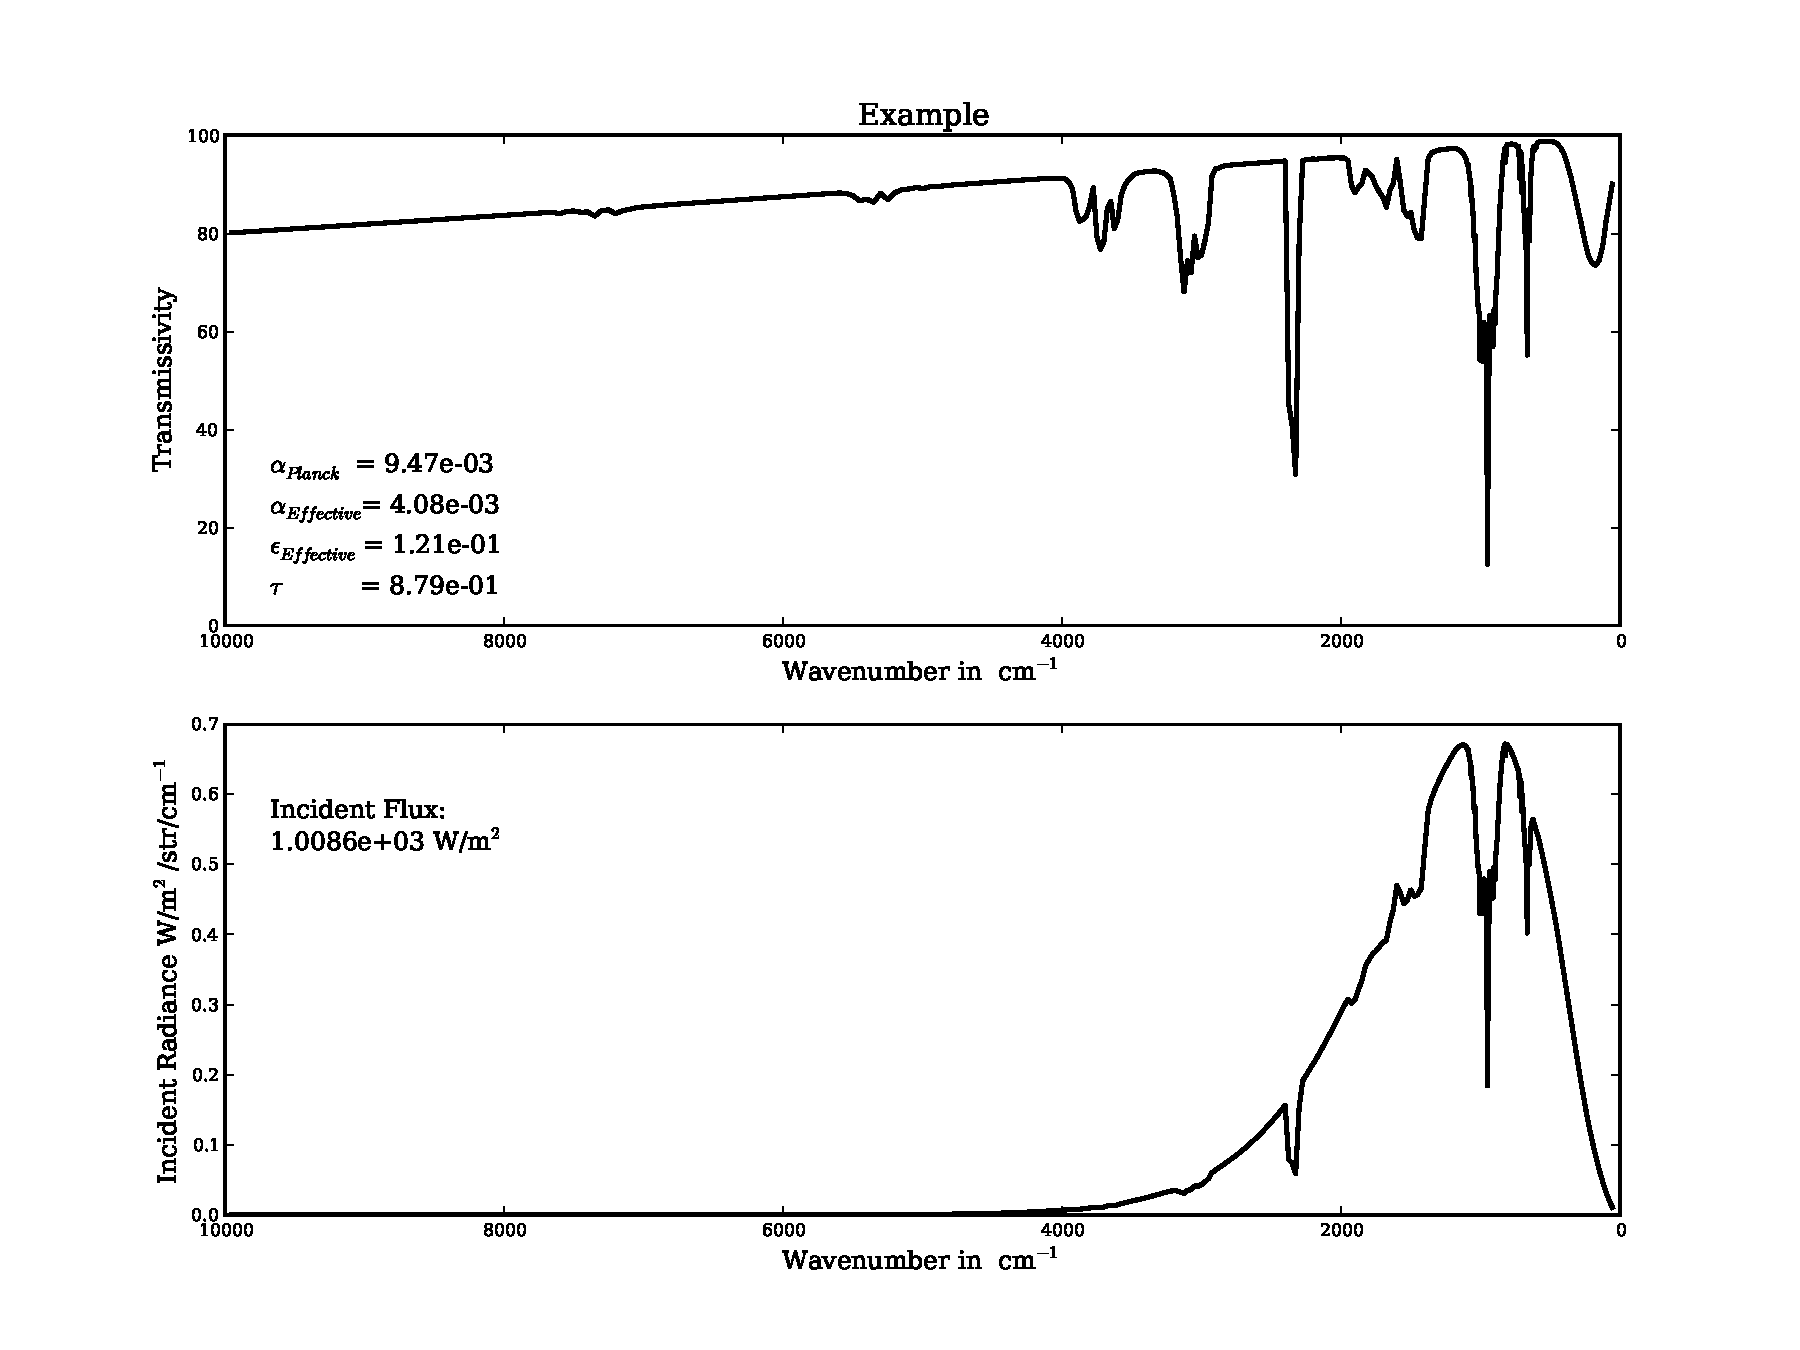
\includegraphics[width=\textwidth]{Figures/Example.pdf}
\caption{Top: Spectral transmissivity of the medium, in \%, using the input file given in Subsection~\ref{sec:input_file}. Bottom: Associated incident spectral intensity, $I_{\om_0}(s)$, given in $\rm W/m^{2}/str/cm^{-1}$.\label{fig:EXAMPLE}}
\end{figure}
